% Journal Article
% LaTeX Template
% Version 2.0 (February 7, 2023)
%
% This template originates from:
% https://www.LaTeXTemplates.com
%
% Author:
% Vel (vel@latextemplates.com)
%
% License:
% CC BY-NC-SA 4.0 (https://creativecommons.org/licenses/by-nc-sa/4.0/)
%
% NOTE: The bibliography needs to be compiled using the biber engine.
%
%%%%%%%%%%%%%%%%%%%%%%%%%%%%%%%%%%%%%%%%%

%----------------------------------------------------------------------------------------
%	PACKAGES AND OTHER DOCUMENT CONFIGURATIONS
%----------------------------------------------------------------------------------------

\documentclass[
	letterpaper, % Paper size, use either a4paper or letterpaper
	12pt, % Default font size, can also use 11pt or 12pt, although this is not recommended
	unnumberedsections, % Comment to enable section numbering
	twoside, % Two side traditional mode where headers and footers change between odd and even pages, comment this option to make them fixed
]{LTJournalArticle}

\addbibresource{bibliography.bib} % BibLaTeX bibliography file

\runninghead{Manipulative Language Detection in LLM-Crafted Phishing Attacks} % A shortened article title to appear in the running head, leave this command empty for no running head

\footertext{\textit{Final Project} (MICS/DATSCI 266, Summer 2025)} % Text to appear in the footer, leave this command empty for no footer text

\setcounter{page}{1} % The page number of the first page, set this to a higher number if the article is to be part of an issue or larger work

%----------------------------------------------------------------------------------------
%	TITLE SECTION
%----------------------------------------------------------------------------------------

\usepackage[title,toc,titletoc]{appendix}
\usepackage{titlesec}
\usepackage{lscape}
\usepackage{fontawesome}
\usepackage{subcaption}
\usepackage{subcaption}
\usepackage{courier}
\usepackage[lighttt]{lmodern}



\title{Manipulative Language Detection in LLM-Crafted
Phishing Attacks
}  % Article title, use manual lines breaks (\\) to beautify the layout}

% Authors are listed in a comma-separated list with superscript numbers indicating affiliations
% \thanks{} is used for any text that should be placed in a footnote on the first page, such as the corresponding author's email, journal acceptance dates, a copyright/license notice, keywords, etc
\author{
	Karl-Johan Westhoff \\
	email: \href{mailto:kjwesthoff@berkeley.edu}{kjwesthoff@berkeley.edu} \\
    Neha Dhage \\
	email: \href{mailto:neha_dhage@ischool.berkeley.edu}{neha\_dhage@ischool.berkeley.edu}
}


% Affiliations are output in the \date{} command
\date{UC Berkeley School of Information \\
MIDS Course 266 Summer 2025 Section 2 (Natalie Ahn) \\
}

% % Full-width abstract
% \renewcommand{\maketitlehookd}{%
% 	\begin{abstract}
% 		\noindent Lorem ipsum dolor sit amet,rta porttitor.
% 	\end{abstract}
% }

%----------------------------------------------------------------------------------------
\setcounter{tocdepth}{5}
\setcounter{secnumdepth}{5}
\usepackage[title]{appendix}

\begin{document}
\maketitle % Output the title section
%----------------------------------------------------------------------------------------
%	ARTICLE CONTENTS
%----------------------------------------------------------------------------------------
\section{Introduction}
The human factor remains central in cyber attacks. The 2024 Verizon DBIR report \cite{verizon2024dbir} notes that 68\% of breaches involve the human element, with phishing as a key contributor. With LLM tools, bad actors can now craft highly convincing phishing messages that evade traditional detection.
This project investigates whether NLP models can detect manipulative language—specifically, text designed to influence actions not in the reader's best interest.

Machine learning (ML) models like Naive Bayes and basic neural networks are widely used to filter email traffic for spam (which is an abundant problem). However, they are often limited to detecting specific words or obvious patterns. Newer approaches combine lightweight ML filtering with resource-heavy NLP methods for cases that are not clearly categorized by simpler filtering. Since phishing often exploits human psychology through language, this study focuses on detecting manipulative language and whether such detection may improve defenses against phishing. Although the focus is on cybersecurity, manipulative language also appears in areas such as coercive or abusive communication, highlighting its broader relevance. Our approach first models manipulation using the “$MentalManip$” dataset, then explores its potential for phishing detection.

\section{Literature}
Salloum et al. \cite{SALLOUM202119} provide an overview of current ML and NLP methods used for phishing detection, which forms the foundational context for this project.
Suhaima et al. \cite{ImprovedPhishing} trained models like BERT on spam data, whereas our focus will be on specifically detecting manipulative language.
Wang et al. \cite{MentalManip} created a data set aiming at dialogue manipulation, which will serve as our primary training set.
Al-Subaiey et al. have compiled a large corpus of emails in \cite{PhishingEmailDataset} from various datasets, under phishing-specific email body texts; this will be used for attempts to detect phishing texts.

\section{Datasets}
Labeled data sets focused on manipulation are rare. Most of the research has come from psychology, which provides insight into the techniques used for manipulation rather than bulk data suitable for AI model training. Most existing data sets suitable for NLP applications are concerned with hate speech and abusive language, which has been an important topic in relation to social media.

\section{"MentalManip" Dataset}
Wang et al. \cite{MentalManip} introduced the "MentalManip" dataset, published on hugging face \cite{MentalManipDataset}. The data set is based on fictional dialogues from "The Cornell Movie Dialogs Corpus" \cite{CornellMovieCorpus} from which suitable manipulative dialogues were selected using BERT and GPT-4 models, from these, 4000 dialogues were manually selected to form the data set. The data is labeled with a detailed manipulation taxonomy in three dimensions; see Figure \ref{fig:Taxonomy}, adding applied technique and psychological vulnerability mechanism to the binary presence of whether the dialogue contains manipulation or not. Some examples of dialogues are listed in appendix \ref{appendix:DialogueExamples}.

\begin{figure}[!htp] % Single column :figure	
	\centering
	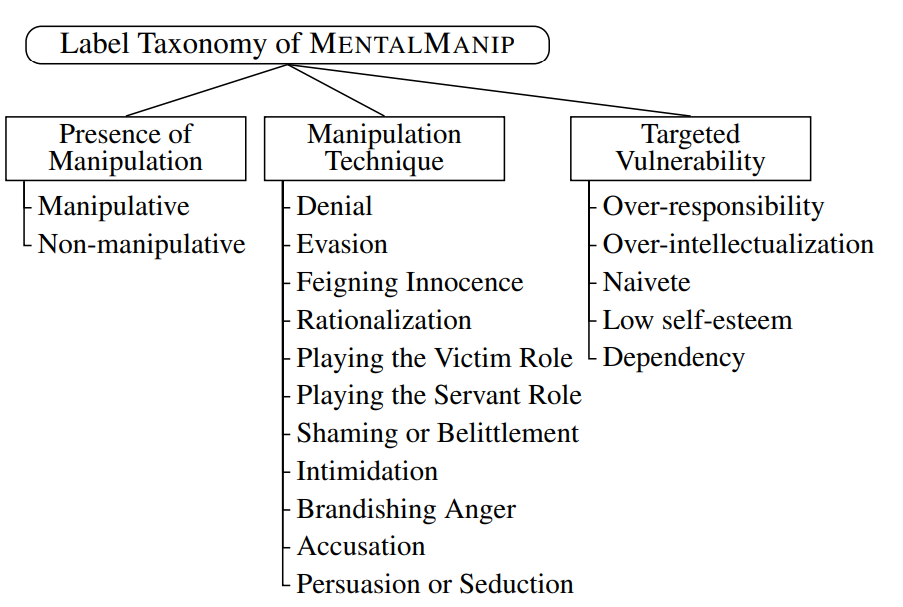
\includegraphics[width=0.5\textwidth]{Taxonomy.png}
	\caption{Taxonomy labels in the data set}
	\label{fig:Taxonomy}
\end{figure}

The data set was manually labeled using a multi-phase human annotation process, adapting the taxonomy (Figure \ref{fig:Taxonomy}) to the dialogue context three times by different people annotating. This gave two versions of the data set, one where the majority two out of three constitutes the result ("$MentalManip_{maj}$") and one where all three annotators have consensus and reach the same results ("$MentalManip_{con}$"). The $MentalManip_{maj}$ data set is larger with 4000 rows and was chosen for this project (The larger size is assumed better for training). We ensured that the dialogues could (mostly) fit into the BERT model embedding size of 512 tokens.
Data exploration can be found in appendix \ref{appendix:DataExploration}

\subsection{Labels}
The dataset features a complex labeling scheme based on the taxonomy in Figure \ref{fig:Taxonomy}. The labels are unevenly distributed, with 'Manipulative' occurring 2.4 times more often than 'Non-manipulative'. Some 'Manipulation Technique' and 'Targeted Vulnerability' labels contain multiple comma-separated values, while others are missing. The co-occurrence of multiple 'Manipulation Technique' labels is shown in Figure \ref{fig:TechCoOcurrence} (see further analysis in Appendix \ref{appendix:Labels}). For phishing detection, we focused on the 'Persuasion and Seduction' label, which is the most frequent in the data (Figure \ref{fig:TechCoOcurrence}). However, using this label for binary inference results in a skewed dataset, with 4.2 times more non-occurrences than occurrences of the label.

\begin{figure}[!htp] % Single column :figure	
	\centering
	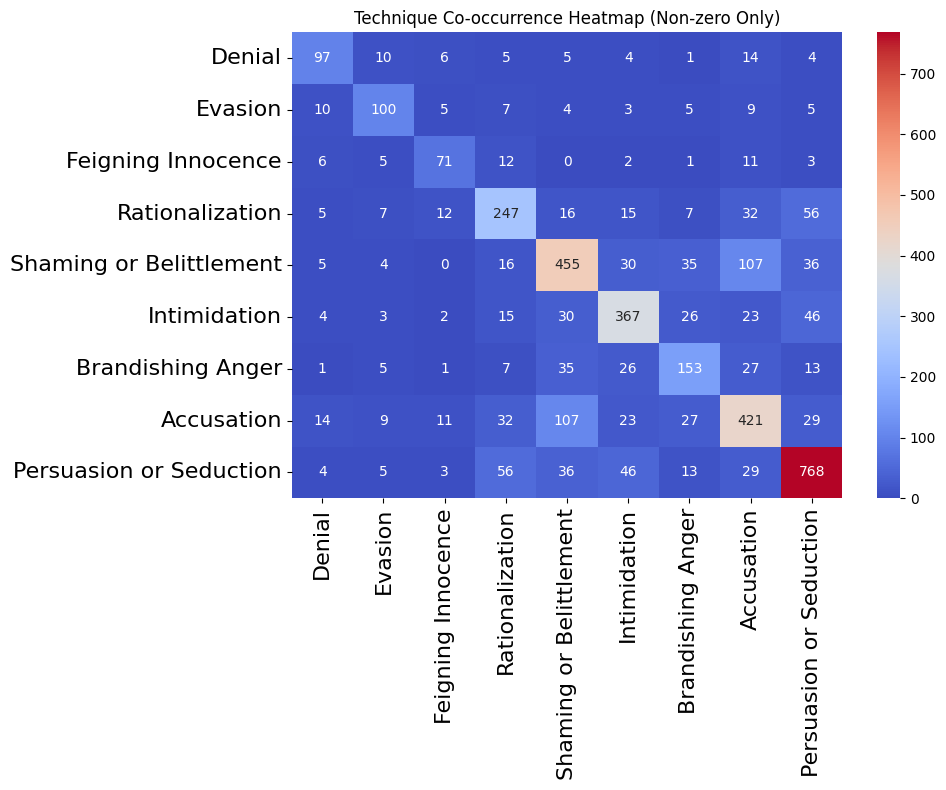
\includegraphics[width=0.5\textwidth]{TechniqueCoOcurrence.png}
	\caption{Distribution and Co-ocurrence of 'Manipulation Technique' labels}
	\label{fig:TechCoOcurrence}
\end{figure}







\section{Baselines}
Given the short embeddings (see Appendix \ref{appendix:DataExploration}), basic BERT models are sufficient for the data. Due to label inconsistencies, we will focus on binary classification of 'Presence of Manipulation' as the baseline for further experimentation.


\subsection{Binary with BERT and its Buddies}
Models looking at the 'manipulative' labels are trained on the $MentalManip_{maj}$ data set. The models were run with similar parameters, and the Accuracy at epoch before significant over fitting\footnote{Significant over fitting defined as: training loss / evaluation loss < 0.6} recorded. Following models were investigated:
\begin{itemize}
	\item BERT-base \cite{BERT-base}
	\item RoBERTa \cite{RoBERTa}
	\item DistilBERT \cite{DistilBERT}
	\item ModernBERT \cite{ModernBERT}
	\item DeBERTaV3 \cite{DeBERTaV3}
\end{itemize}
Furthermore some "emotionally wiser" BERT derivatives exist which are pre-trained for emotion detection:
\begin{itemize}
	\item BERTweet \cite{BERTweet}
	\item EmotionBERT \cite{EmotionBERT}
\end{itemize}

\subsection{Baseline Results and Discussion}\label{sec:BaselineResults}
Results with losses and accuracy are shown in Table \ref{tab:BaseModelPerformance}. The models were run until significant over-fitting occurred. In general the models over-fit after a few epochs which is to be expected with a model that is extended from pre-trained. The Accuracy results are around 0.70-0.72 with little variation. Models can be found in Appendix \ref{appendix:BaseCaseModels}

\subsubsection{ModernBERT} The model does not perform better, this was expected as the embedding lengths are short (see Figure \ref{fig:DialogueEmbedding}) and not leveraging the benefits of ModernBERTs larger capacity.

\subsubsection{Emotionally intelligent BERT}
BERTweet performs on par with BERT-base, the model is primarily trained for "Part-of-speech tagging", "Named-entity recognition" and "text classification" \cite{BERTweet} herunder including emjojis etc. i.e. The model is not per-se expected to be better at manipulation detection, but we decided to give it a try since the EmotionBERT model was created for multi label classification of well known emotional phrases for media monitoring \cite{EmotionBERT}.

\subsubsection{Advanced BERTs}
We also tried some more advanced BERT derivatives (DestilBERT and deBERTa\_v3\_small), however these models did not perform better than RoBERTa, and they required more compute resources to train. DeBERTa uses more advanced training loss, pre-training more advanced encoding etc.\cite{DeBERTaV3}, however only the smallest version of deBERTa was possible to train with the hardware available. These models are optimized to deliver faster inference, but the extra cost in training resources make them less feasible for this project.
\subsubsection{RoBERTa}
The second best performing model reported in Table \ref{tab:BaseModelPerformance} was RoBERTa, which seems to perform slightly better than BERT-base, however with multiple tries the performance was not consistent, sometimes BERT performed better, however RoBERTa seemed more stable giving consistent results above 0.72 and performing more Epochs before over-fitting.


\begin{table}[h!]
	\small
	\begin{tabular}{|p{2.2cm}|p{0.9cm}|p{1cm}|p{1cm}|p{1cm}|}
		\hline
		\textbf{Model} & \textbf{Epoch} & \textbf{Loss T/V} & \textbf{Acc Epoch} & \textbf{Acc Final} \\
		\hline
		BERT           & 2              & 0.97              & 0.726              & 0.70               \\
		roBERTa        & 4              & 1.03              & 0.728              & 0.73               \\
		deBERTa\_v3    & 3              & 0.68              & 0.704              & 0.72               \\
		DistilBERT     & 2              & 0.75              & 0.709              & 0.72               \\
		ModernBERT     & 2              & 0.81              & 0.718              & 0.72               \\
		BERTweet       & 2              & 0.97              & 0.705              & 0.70               \\
		EmotionBERT    & 2              & 1.04              & 0.712              & 0.74               \\


		\hline
	\end{tabular}
	\caption{Base Model performance comparison across different transformer architectures for binary inference on the "manipulative" column: Epochs before significant over-fitting, Training loss / Validation loss (to measure  overfitting) and accuracy at epoch and final classification }
	\label{tab:BaseModelPerformance}
\end{table}

\section{Fine Tuning}
Based on the results in section \ref{sec:BaselineResults}, we decided to fine tune the RoBERTa model with the $MentalManip_{maj}$ data set to see if we can get better results for the manipulation detection task. The MentalManip article\cite{MentalManip} achieved an accuracy of 0.78.

\subsection{LoRA/PEFT}
We applied LoRA technique to 
\subsection{Hyper parameters}







\section{Experiments}
Persuasion is expected to be the main technique in phishing, where the aim is to get people to take some action on behalf of the attacker. Therefore we will focus on the 'persuasion' label in our experiments.

\subsection{Persuasion}
\subsubsection{Feature Engineering}
The 'technique' column in the data set was chosen as binary label, with 'persuasion' present in the text being the positive class (some rows have multiple technique labels). The label distribution is 4.2 to 1 for the 'non-persuasion' to 'persuasion' labels, i.e. near the opposite of the data sets 'manipulative' vs 'not' when including all techniques and vulnerabilities.

\subsubsection{Results and Discussion, Persuasion}
Classification Report for the 'Persuasion' label, Base Case un-weighted is shown in Table \ref{tab:BaseCasePersuasionReport}. At a glance, the model shows decent overall accuracy (0.80), However as we are interested in identifying persuasion the important metrics are recall and precision for the 'Manipulative' class, here the results are not so impressive, out of all actual manipulative instances, only 28\% were correctly predicted as manipulative (confusion matrix and results are shown in appendix \ref{fig:UNWeightedResults}). The cause for the models difficulty identifying persuasion is assumed to be the skewed label distribution.

\begin{table}[h!]
	\small
	\centering
	\begin{tabular}{|p{2.2cm}|p{1cm}|p{1cm}|p{1cm}|c|c|c|}
		\hline
		\textbf{Class}     & \textbf{Prec.} & \textbf{Rec.} & \textbf{F1} & \textbf{Sup.} \\
		\hline
		Non-manip.         & 0.85           & 0.92          & 0.88        & 649           \\
		\hline
		Manipulative       & 0.46           & 0.28          & 0.35        & 151           \\
		\hline
		\hline
		\textbf{Accuracy}  &                &               & 0.80        & 800           \\
		\hline
		\textbf{Macro avg} & 0.65           & 0.60          & 0.61        & 800           \\
		\hline
		\textbf{Wght. avg} & 0.77           & 0.80          & 0.78        & 800           \\
		\hline
	\end{tabular}
	\caption{Classification Report for the 'Persuasion' label, Base Case un-weighted}
	\label{tab:BaseCasePersuasionReport}
\end{table}

\subsection{Weighted loss function}

To remedy the skewed label distribution, a suggested approach is adding weights to the loss function, suppressing the majority and boosting the minority class. Alternatives are over- and under-sampling. Under-sampling was disregarded due to the limited dataset size of 4,000 rows, as it would further reduce the available training data and risk losing information. Oversampling was considered but ultimately avoided to prevent overfitting, particularly since duplicating minority samples can lead the model to remember specific sentences. Zhang et al. \cite{zhang2020revisiting} suggests that weighting the loss function is more effective than sampling when fine-tuning BERT on imbalanced data. \\

Weights are calculated based on the label distribution and applied to the cross-entropy loss function during training\footnote{A custom derivative of the Trainer class was implemented, see links to notebooks in Appendix \ref{appendix:WeightedResults}}. We tried a number of schemes to determine weights:
\begin{enumerate}
	\item Weights inversely proportional to the class distribution, see Figure \ref{fig:V1WeightDistributionRaw}
	\item Weights inversely proportional to the class distribution but max weight capped at 4.0 and 3.0 respectively
	\item Weights normalized to add up to 1
\end{enumerate}



\begin{figure}[h]
	\centering
	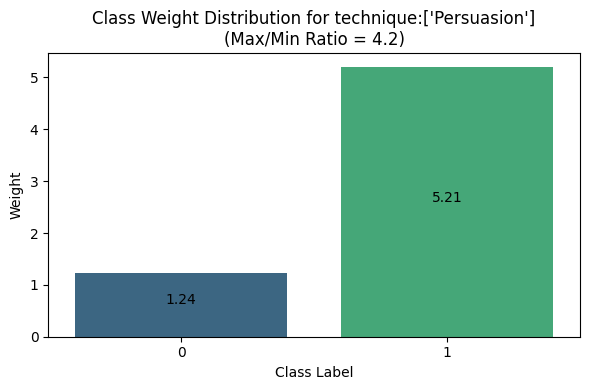
\includegraphics[width=0.5\textwidth]{WeightDistributionV1.png}
	\caption{Distribution of weights for the Persuasion label, no modifications to the weight distribution}
	\label{fig:V1WeightDistributionRaw}
\end{figure}%

\begin{figure}[h]
	\centering
	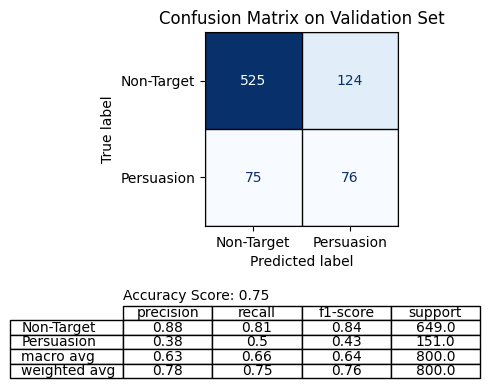
\includegraphics[width=0.5\textwidth]{WeightedV1Results.png}

	\caption{Results for un-capped and un-normalized weighted cross-entropy loss function}
	\label{fig:V1WeightResultsRaw}
\end{figure}%

\subsubsection{Results and Discussion, Weighted Models}
The un-capped un-normalized option 1 version performed best, Results are shown in Figure \ref{fig:V1WeightResultsRaw}. Option 1 adds the most weight to the minority class and gives a recall of 0.5 for the 'Manipulative' class improving the un-weighted result in Table \ref{tab:BaseCasePersuasionReport}, however the model still only gets 38\% of the manipulative cases correct, with high false positives. Results for option 2 and 3 give slightly lower recalls in proportion to the lower weights added to the minority label and better overall Accuracy results (favoring the non manipulative class). Results are shown in Appendix \ref{appendix:WeightedResults}. \\
An observed feature during training, shown in Figure \ref{fig:V1EpochPlot}, epochs 2-4 with decreasing training loss, increasing validation loss while F1 and recall scores still show a positive trend. This is likely due to the model over fitting the majority class, however for this application we are interested in the minority class, so recall and F1 are better metrics for detecting "over fitting of the minority class".

\begin{figure}[h]
	\centering
	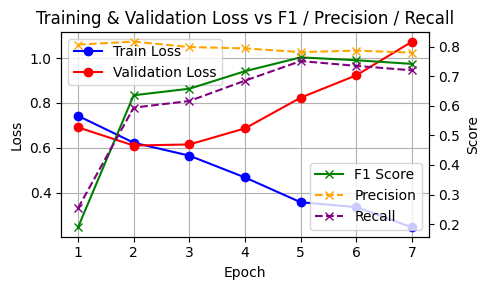
\includegraphics[width=0.5\textwidth]{LossesVsF1_V1.png}
	\caption{Losses and Results vs epochs (Note: the model is allowed to run beyond overfit at epoch 3 fowr illustration)}
	\label{fig:V1EpochPlot}
\end{figure}%







\section{Conclusion}

The baseline investigations showed that applying the $MentalManip$ dataset to models optimized for emotional language detection does not automatically improve accuracy. Mental manipulation is less explored in literature than hate speech and abusive language, which are key concerns in social media, where sentiment analysis is both established and evolving in NLP, using these models do not directly translate to improvement in detecting manipulation. \\
Investigating 'persuasion' as a means for detecting Phishing, requires some model manipulation as we are trying to detect a minority class, and the results show moderate (at best) viability for detecting persuasion.

The MentalManip article \cite{MentalManip} also uses some decoder only models by 'zero' and 'few-shot' prompting the model with random example from the data set. This seems to perform better for overall binary classification, but only a little, and the LLM's have a tendency to pick up on toxicity and hate-speech and identify these as manipulation.


%----------------------------------------------------------------------------------------
%	 REFERENCES
%----------------------------------------------------------------------------------------
\clearpage
\onecolumn
\printbibliography % Output the bibliography
%----------------------------------------------------------------------------------------

%----------------------------------------------------------------------------------------
%	 Appendices
%---------------------------------------------------------------------------------------
\appendix
\counterwithin{figure}{section}

\begin{appendices}
	\onecolumn
	%
	\section{Data Exploration}\label{appendix:DataExploration}

	\subsection{Dialogues}
	The 4000 dialogues in the data set are between two persons exchanging sentences. Word count statistics are shown in Figure \ref{fig:DialogueWordCount}, most dialogues consist of up to 50 words per person, and the number of words uttered by each person is fairly balanced, with person 2 saying slightly more words than person 1 in the up to 50 word majority case. Figure \ref{fig:DialogueEmbedding} shows the distribution of token counts for the dialogues in the data set, tokenized using BERT-base as reference. Only a minor number of dialogues exceed the BERT-base embedding size of 512 tokens.


	\begin{figure}[!htp] % Single column :figure	
		\centering
		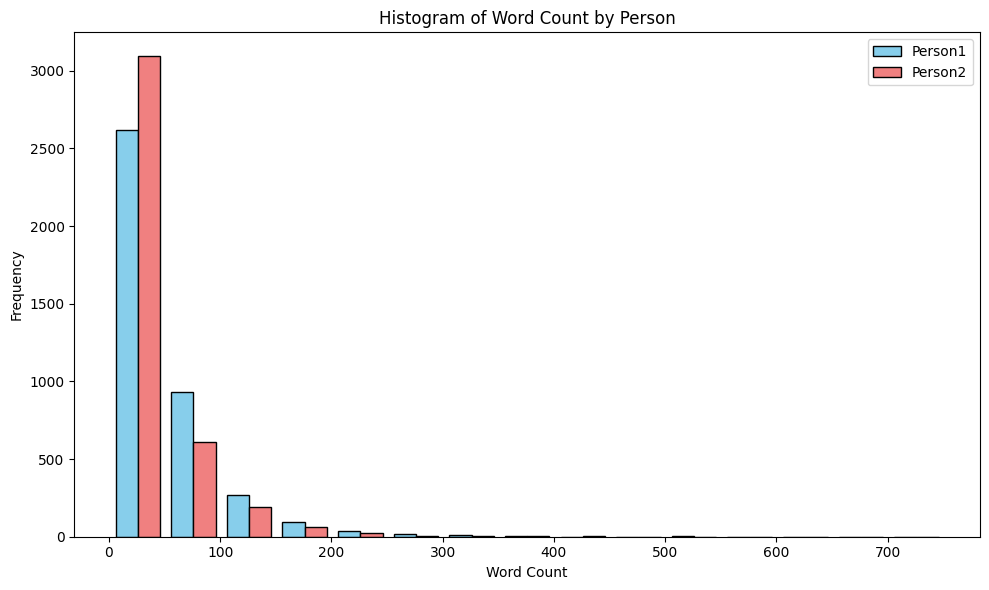
\includegraphics[width=0.5\textwidth]{DialogueWordCountStats.png}
		\caption{Word count statistics for the dialogues in the $MentalManip_{maj}$ data set, words uttered by each person}
		\label{fig:DialogueWordCount}
	\end{figure}

	\begin{figure}[!htp] % Single column :figure	
		\centering
		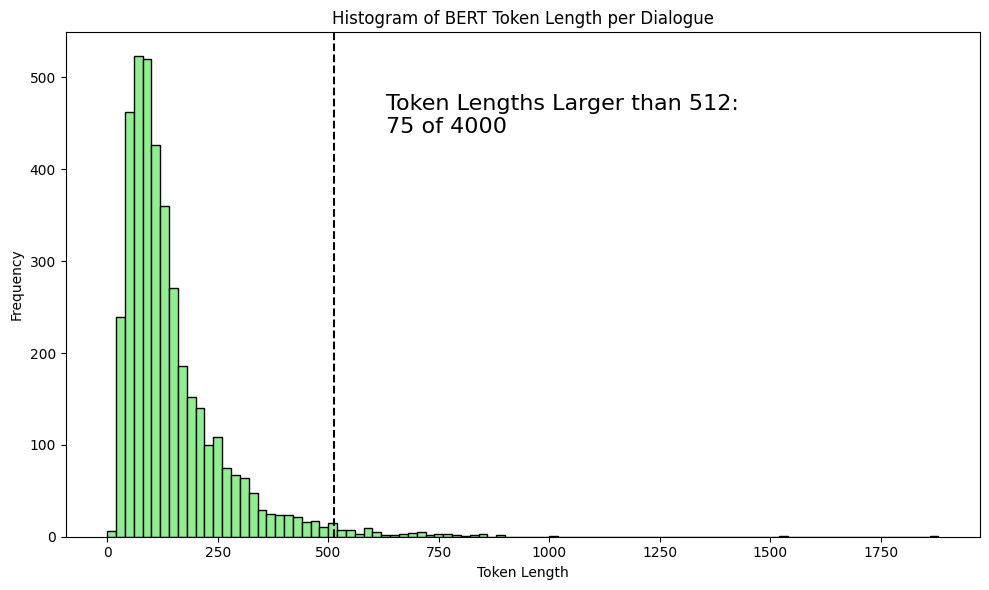
\includegraphics[width=0.5\textwidth]{DialogueEmbeddingStats.png}
		\caption{Statistics for the dialogue in the $MentalManip_{maj}$ data set, tokenized using BERT-base}
		\label{fig:DialogueEmbedding}
	\end{figure}


	\subsection{Labels}\label{appendix:Labels}

	\subsubsection{Manipulation Label}
	The data set is not split equally between manipulation and non-manipulation, Figure \ref{fig:ManipulationRatio} shows the distribution with 2.4 times more manipulation rows than non-manipulation.

	\begin{figure}[!htp] % Single column :figure	
		\centering
		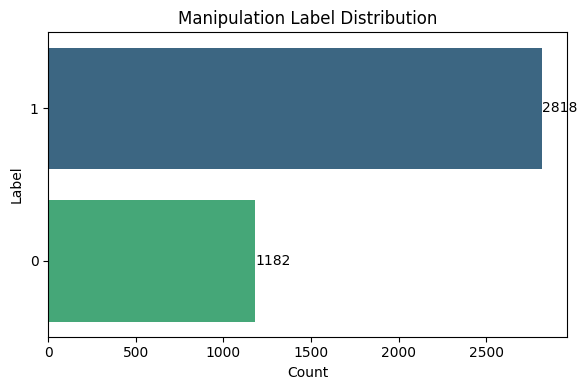
\includegraphics[width=0.5\textwidth]{ManipulationRatio.png}
		\caption{Ratio of manipulation to non-manipulation in the $MentalManip_{maj}$ Dataset}
		\label{fig:ManipulationRatio}
	\end{figure}

	\subsubsection{'Technique' and 'Vulnerability' Labels}
	Some of the labels are missing for some of the rows with manipulation present\footnote{The labels should not be populated for non-manipulation rows}, Figure \ref{fig:MissingLabels} shows a total of 664\footnote{110 missing technique and 554 also missing vulnerability} missing labels for 'technique', we regard the technique labels as most relevant for phishing, especially the 'Persuasion or Seduction' label.
	\begin{figure}[!htp] % Single column :figure	
		\centering
		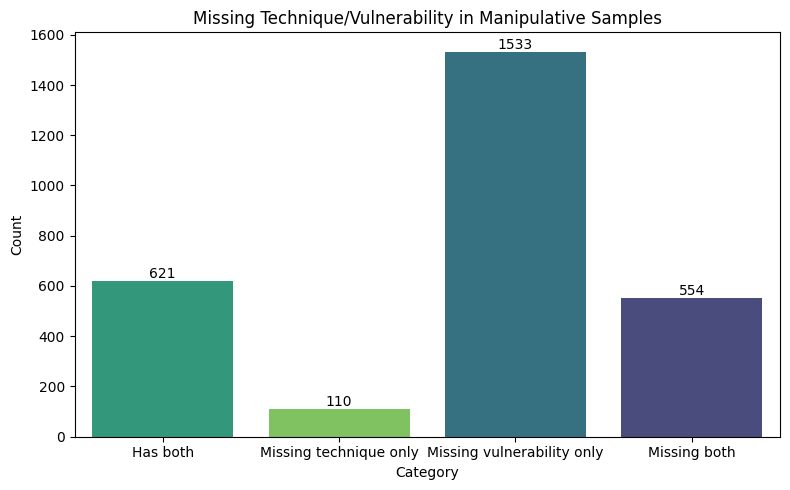
\includegraphics[width=0.5\textwidth]{MisingLabels.png}
		\caption{Incomplete labeling of the MentalManip Dataset}
		\label{fig:MissingLabels}
	\end{figure}







	\url{https://github.com/KJWesthoff/266FinalProject/blob/main/Data-Exploration_MentalManip.ipynb}

	\section{BaseCaseModels}\label{appendix:BaseCaseModels}
	\url{https://github.com/KJWesthoff/266FinalProject/tree/main/BaseCaseModels}

	\section{'Persuasion' Experiments}\label{appendix:PersuasionExperiments}
	\subsection{Label distribution}\label{appendix:PersuasionLabelDistribution}
	\begin{figure}[!htp] % Single column :figure	
		\centering
		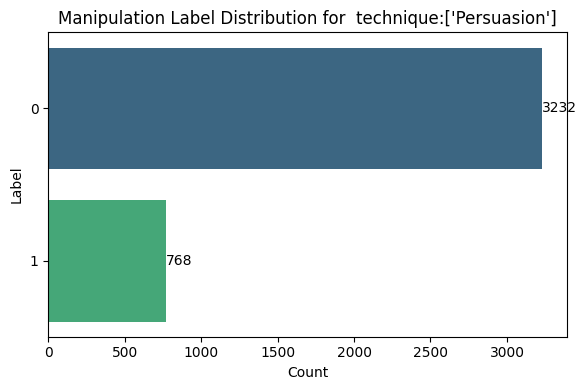
\includegraphics[width=0.5\textwidth]{PersuasionLabelDistribution.png}
		\caption{Label distribution with a 4.2 to 1 ratio for the 'not-persuation' to  'persuasion' labels in the $MentalManip_{maj}$ data set}
		\label{fig:PersuasionLabelDistribution}
	\end{figure}


	\subsection{Baseline Results, Un-Weighted}\label{appendix:UnWeightedResults}
	Notebook here:
	\url{https://github.com/KJWesthoff/266FinalProject/blob/main/WeightedSkew/RoBERTa_Binary_ManipDetection_PersuasionBinary_Un-Weighted.ipynb}



	\begin{figure*}[t!]
		\centering
		\begin{subfigure}[t]{0.5\textwidth}
			\centering
			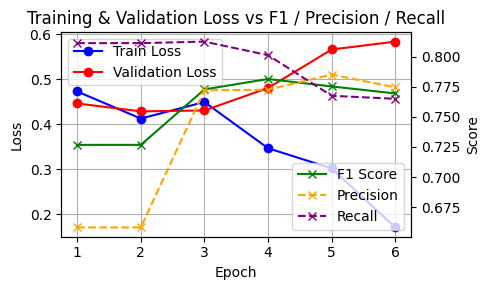
\includegraphics[height=0.5\textwidth]{LossesVsF1_Unweighted.png}
			\caption{Losses and Results vs epochs for the un-weighted model}
			\label{fig:UnWeightedEpochPlot}
		\end{subfigure}%
		~
		\begin{subfigure}[t]{0.4\textwidth}
			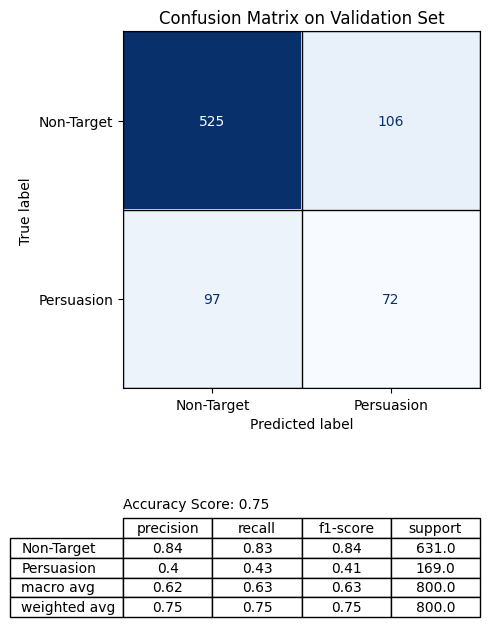
\includegraphics[height=\textwidth]{UnWeightedResults.png}
			\caption{Confusion matrix and classification report for the un weighted Persuasion label base case model}
			\label{fig:UNWeightedResults}
			\centering
		\end{subfigure}
		\caption{Results for the un weighted persuasion label base case model}
	\end{figure*}











	\subsection{Baseline Results, Weighted}\label{appendix:WeightedResults}
	Notebooks here:
	\url{https://github.com/KJWesthoff/266FinalProject/blob/main/WeightedSkew/RoBERTa_Binary_ManipDetection_PersuasionBinary_WeightedV1.ipynb}
	\url{https://github.com/KJWesthoff/266FinalProject/blob/main/WeightedSkew/RoBERTa_Binary_ManipDetection_PersuasionBinary_WeightedV2.ipynb}
	\url{https://github.com/KJWesthoff/266FinalProject/blob/main/WeightedSkew/RoBERTa_Binary_ManipDetection_PersuasionBinary_WeightedV3.ipynb}


	\begin{figure*}[t!]
		\centering
		\begin{subfigure}[t]{0.5\textwidth}
			\centering
			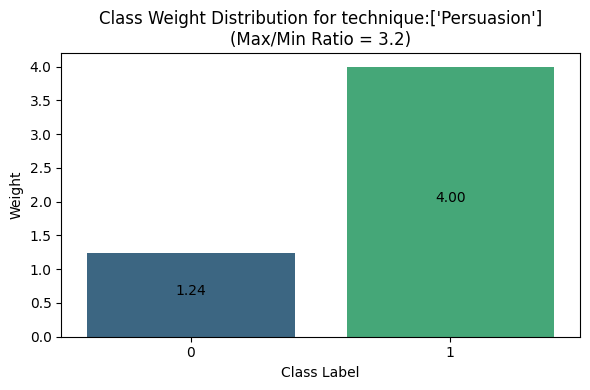
\includegraphics[height=0.5\textwidth]{WeightDistributionV2.png}
			\caption{Distribution of weights for the Persuasion label}
			\label{fig:V2WeightDistribution}
		\end{subfigure}%
		~
		\begin{subfigure}[t]{0.5\textwidth}
			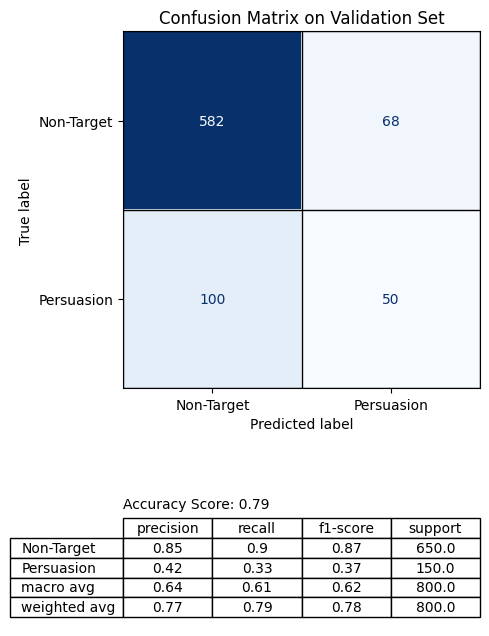
\includegraphics[height=\textwidth]{WeightedV2Results.png}
			\caption{Confusion matrix and classification report for the Persuasion label base case model}
			\label{fig:V2Results}
			\centering
		\end{subfigure}
		\caption{Results for cross entropy weight capped at 4.0}
	\end{figure*}

	\begin{figure*}[t!]
		\centering
		\begin{subfigure}[t]{0.5\textwidth}
			\centering
			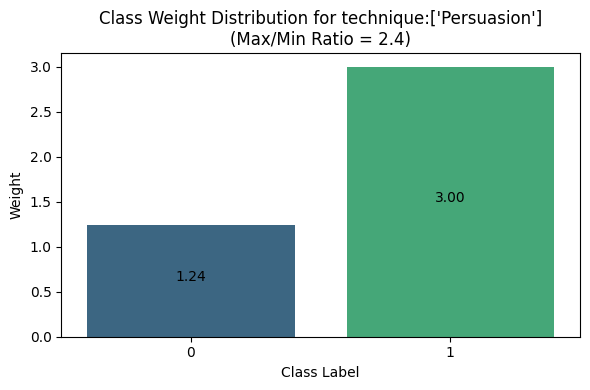
\includegraphics[height=0.5\textwidth]{WeightDistributionV2b.png}
			\caption{Distribution of weights for the Persuasion label}
			\label{fig:V2bWeightDistribution}
		\end{subfigure}%
		~
		\begin{subfigure}[t]{0.5\textwidth}
			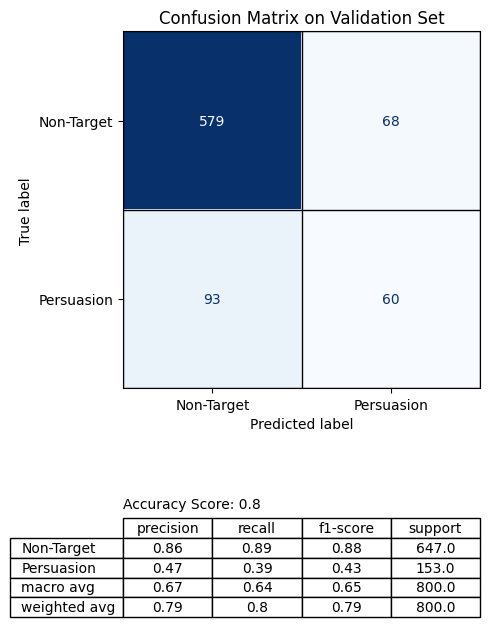
\includegraphics[height=\textwidth]{WeightedV2bResults.png}
			\caption{Confusion matrix and classification report for the Persuasion label base case model}
			\label{fig:V2bResults}
			\centering
		\end{subfigure}
		\caption{Results for cross entropy weight capped at 3.0}
	\end{figure*}


	\begin{figure*}[t!]
		\centering
		\begin{subfigure}[t]{0.5\textwidth}
			\centering
			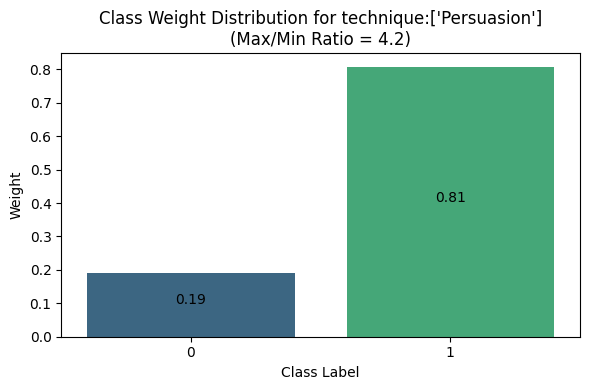
\includegraphics[height=0.5\textwidth]{WeightDistributionV3.png}
			\caption{Distribution of weights for the Persuasion label}
			\label{fig:V3WeightDistribution}
		\end{subfigure}%
		~
		\begin{subfigure}[t]{0.5\textwidth}
			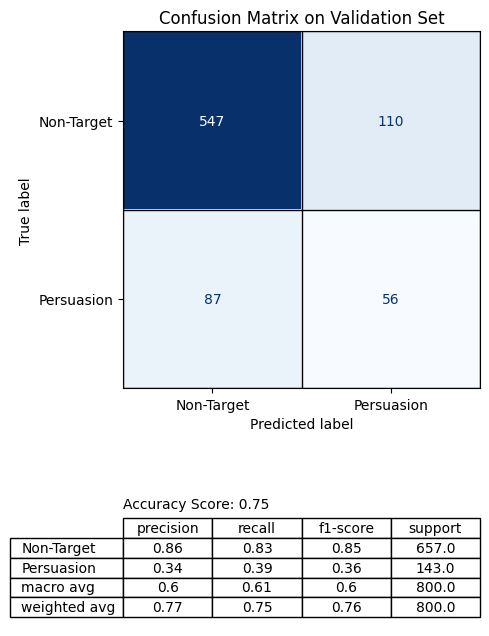
\includegraphics[height=\textwidth]{WeightedV3Results.png}
			\caption{Confusion matrix and classification report for the Persuasion label base case model}
			\label{fig:V3Results}
			\centering
		\end{subfigure}
		\caption{Results for normalized weighted cross-entropy loss function}
	\end{figure*}
	\clearpage
	\section{Dialogue examples}\label{appendix:DialogueExamples}
	\subsection{True Positives:}
	{\ttfamily \tiny
		\noindent\textbf{Person1:}  You're making it too easy. \\
		\noindent\textbf{Person2:}  You got time on your side.  Pretty soon they'll be missed and we'll have the law up our ass. \\
		\noindent\textbf{Person1:}  They saw you kill the driver. \\
		\noindent\textbf{Person2:}  You're up on your details, aren't you? \\
		\noindent\textbf{Person1:}  You can rely on them to keep quiet because this is undeclared money that could land Jack there in federal prison.  He can't afford for you to get caught and have this briefcase appear as evidence. \\
		\noindent\textbf{Person2:}  Keep talking. \\

		\noindent\textbf{Person1:}  Drink this! It will dull your pain. \\
		\noindent\textbf{Person2:}  It will numb my wits, and I must have them all. If I'm senseless, or if I wail, then Longshanks will have broken me. \\
		\noindent\textbf{Person1:}  I can't bear the thought of your torture. Take it! \\


	}

	\subsection{False Negatives:}
	{\ttfamily \tiny
		\noindent\textbf{Person1:}  She's working as fast as she can, Icarus.  It will be ready soon. \\
		\noindent\textbf{Person2:}  It's ready now, I know it is. \\
		\noindent\textbf{Person1:}  She says it's not. \\
		\noindent\textbf{Person2:}  She's lying.  She lost the first one on purpose. \\
		\noindent\textbf{Person1:}  She did not.  The mouse ran down the drain. \\
		\noindent\textbf{Person2:}  She let it escape because she wants me to die. \\
		\noindent\textbf{Person1:}  Don't be a child, Icarus.  She is just another scientist and like all scientists, she doesn't care about anything outside the \\

		\noindent\textbf{Person1:}  Why did you have LUH come here? \\
		\noindent\textbf{Person2:}  Why are you so concerned? \\
		\noindent\textbf{Person1:}  What's going on? \\
		\noindent\textbf{Person2:}  I want you for my roommate. \\
		\noindent\textbf{Person1:}  Where's LUH? \\
		\noindent\textbf{Person2:}  It will be good for both of us. I've got it all arranged. \\


	}

	\subsection{False Positives:}
	{\ttfamily \tiny
		\noindent\textbf{Person1:}  Yes! You own the Coffer of Shadow. Nothing can withstand its power. \\
		\noindent\textbf{Person2:}  I've been saving it. For the right moment. \\
		\noindent\textbf{Person1:}  That moment is now! What good is a sword unless it be unsheathed? Use it, and no one will dare oppose you again. No one. \\

		\noindent\textbf{Person1:}  Here and there. Around. \\
		\noindent\textbf{Person2:}  Uh-huh. One of those cozy bed and breakfast places, probably. \\
		\noindent\textbf{Person1:}  Yeah, that's right. \\
		\noindent\textbf{Person2:}  Except that there's no bed, is there? And no breakfast either. \\
		\noindent\textbf{Person1:}  The material world is an illusion. It doesn't matter if they're there or not. The world is in my head. \\
		\noindent\textbf{Person2:}  But your body is in the world, isn't it?  If someone offered you a place to stay, you wouldn't necessarily refuse, would you? \\
		\noindent\textbf{Person1:}  \\


	}

	\subsection{True Negatives:}
	{\ttfamily \tiny
		\noindent\textbf{Person1:}  I don't know who you think you're talking to! I ain't some whore you brought here! I've been trying to be your friend and you treat me like shit! \\
		\noindent\textbf{Person2:}  Be a friend. Leave. \\
		\noindent\textbf{Person1:}  You got no manners and you never tell the truth! You're nothin' special. And if you ask me, you got no chance at all of being an officer! \\

		\noindent\textbf{Person1:}  Oh, Rufus! \\
		\noindent\textbf{Person2:}  All I can offer you is a Rufus over your head. \\
		\noindent\textbf{Person1:}  Oh, Your Excellency, I don't know what to say. \\
		\noindent\textbf{Person2:}  I wouldn't know what to say either if I was in your place.  Maybe you can suggest something. \\


	}



\end{appendices}
%
\end{document}
